\subsection{Observed PDD Curves}

\begin{figure}[H]
	\centering
	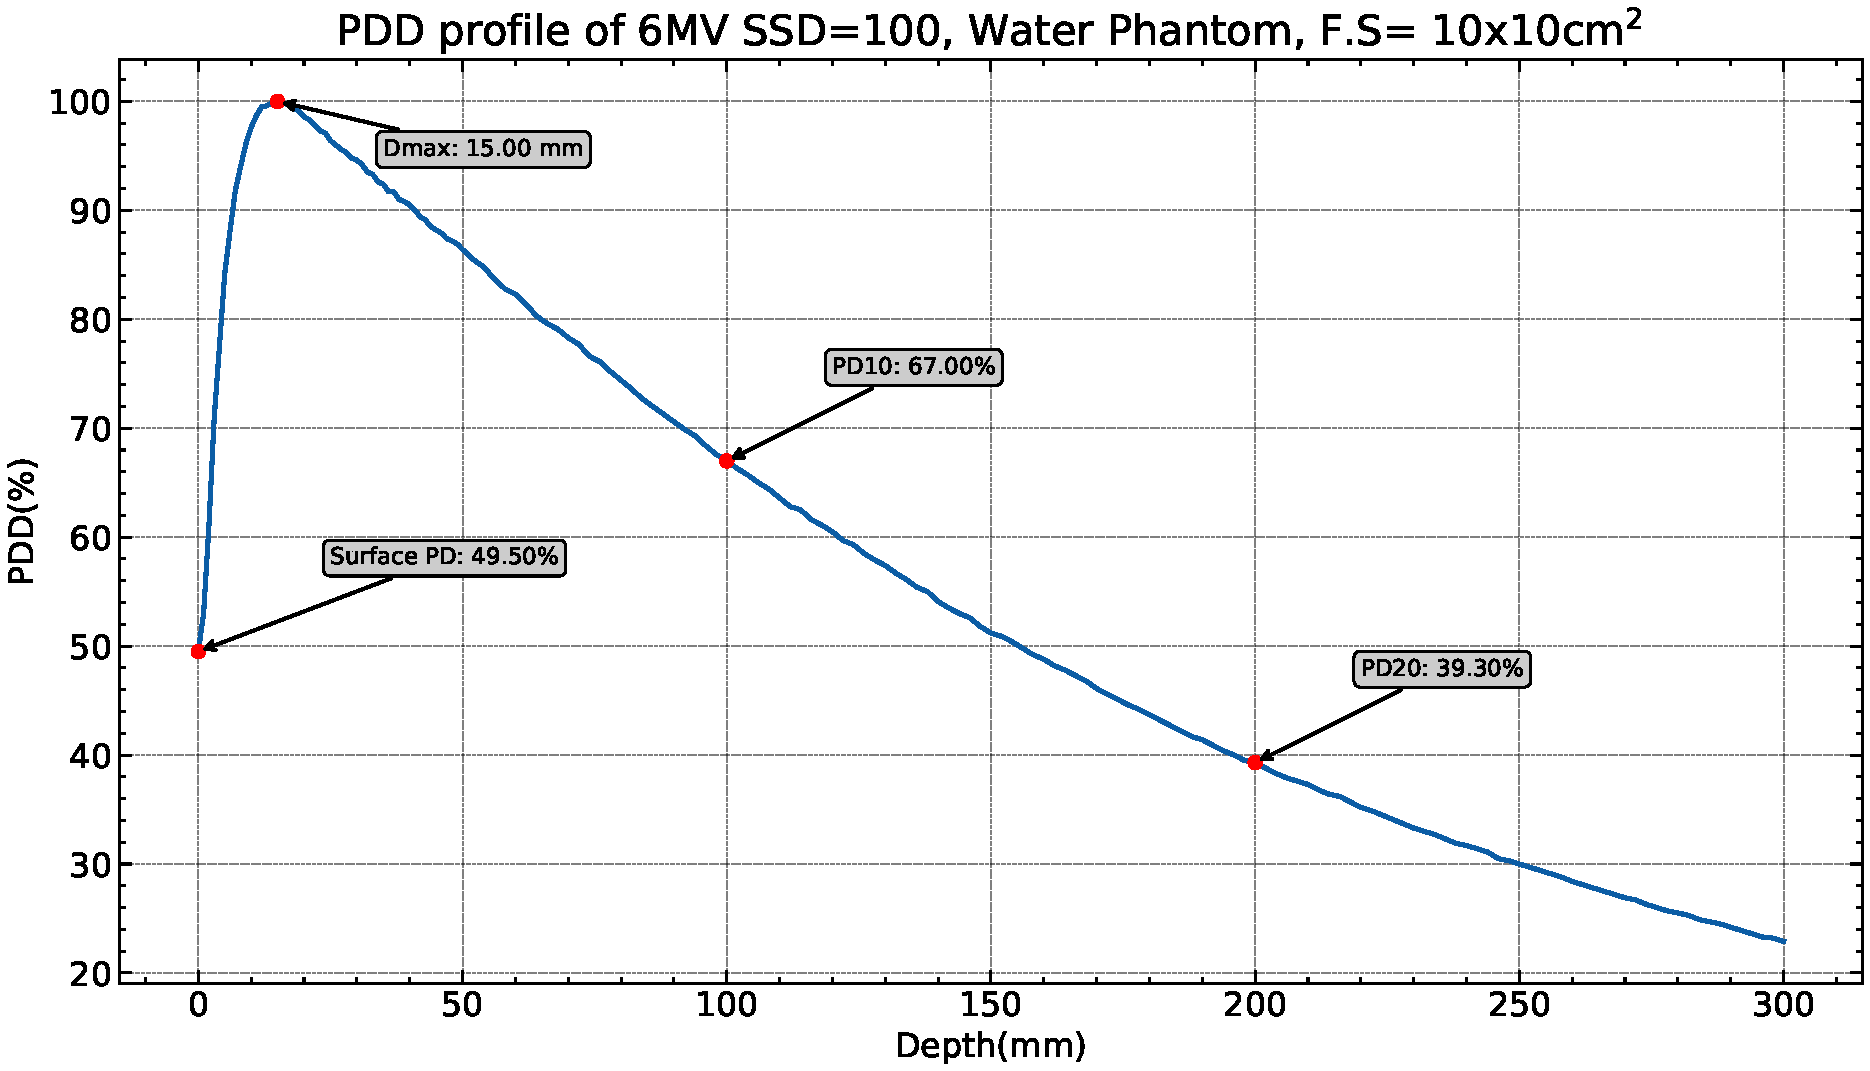
\includegraphics[width=0.8\textwidth]{Program/Figures/PDD/PDD_6MVPhoton.pdf}
	\caption{Percentage depth dose for 6 MV photon beam.}
\end{figure}

\begin{figure}[H]
	\centering
	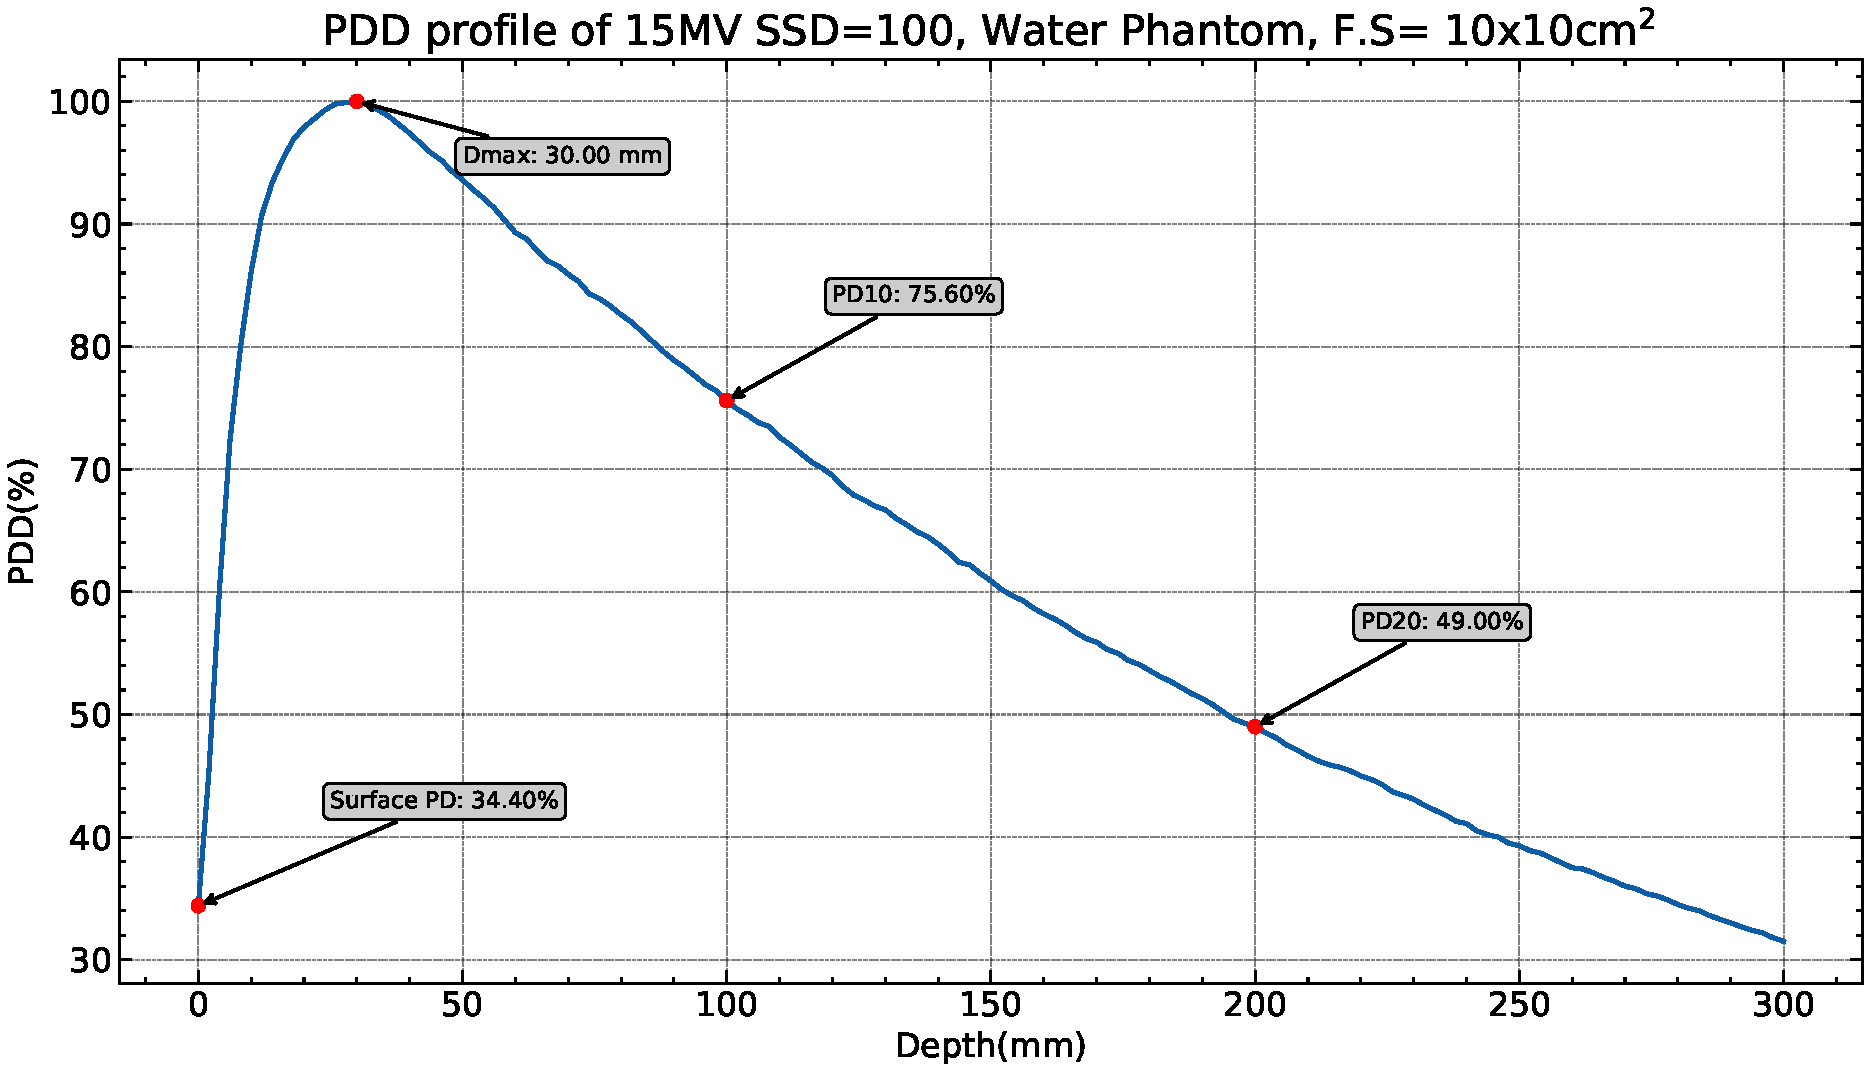
\includegraphics[width=0.8\textwidth]{Program/Figures/PDD/PDD_15MVPhoton.pdf}
	\caption{Percentage depth dose for 15 MV photon beam.}
\end{figure}

\begin{figure}[H]
	\centering
	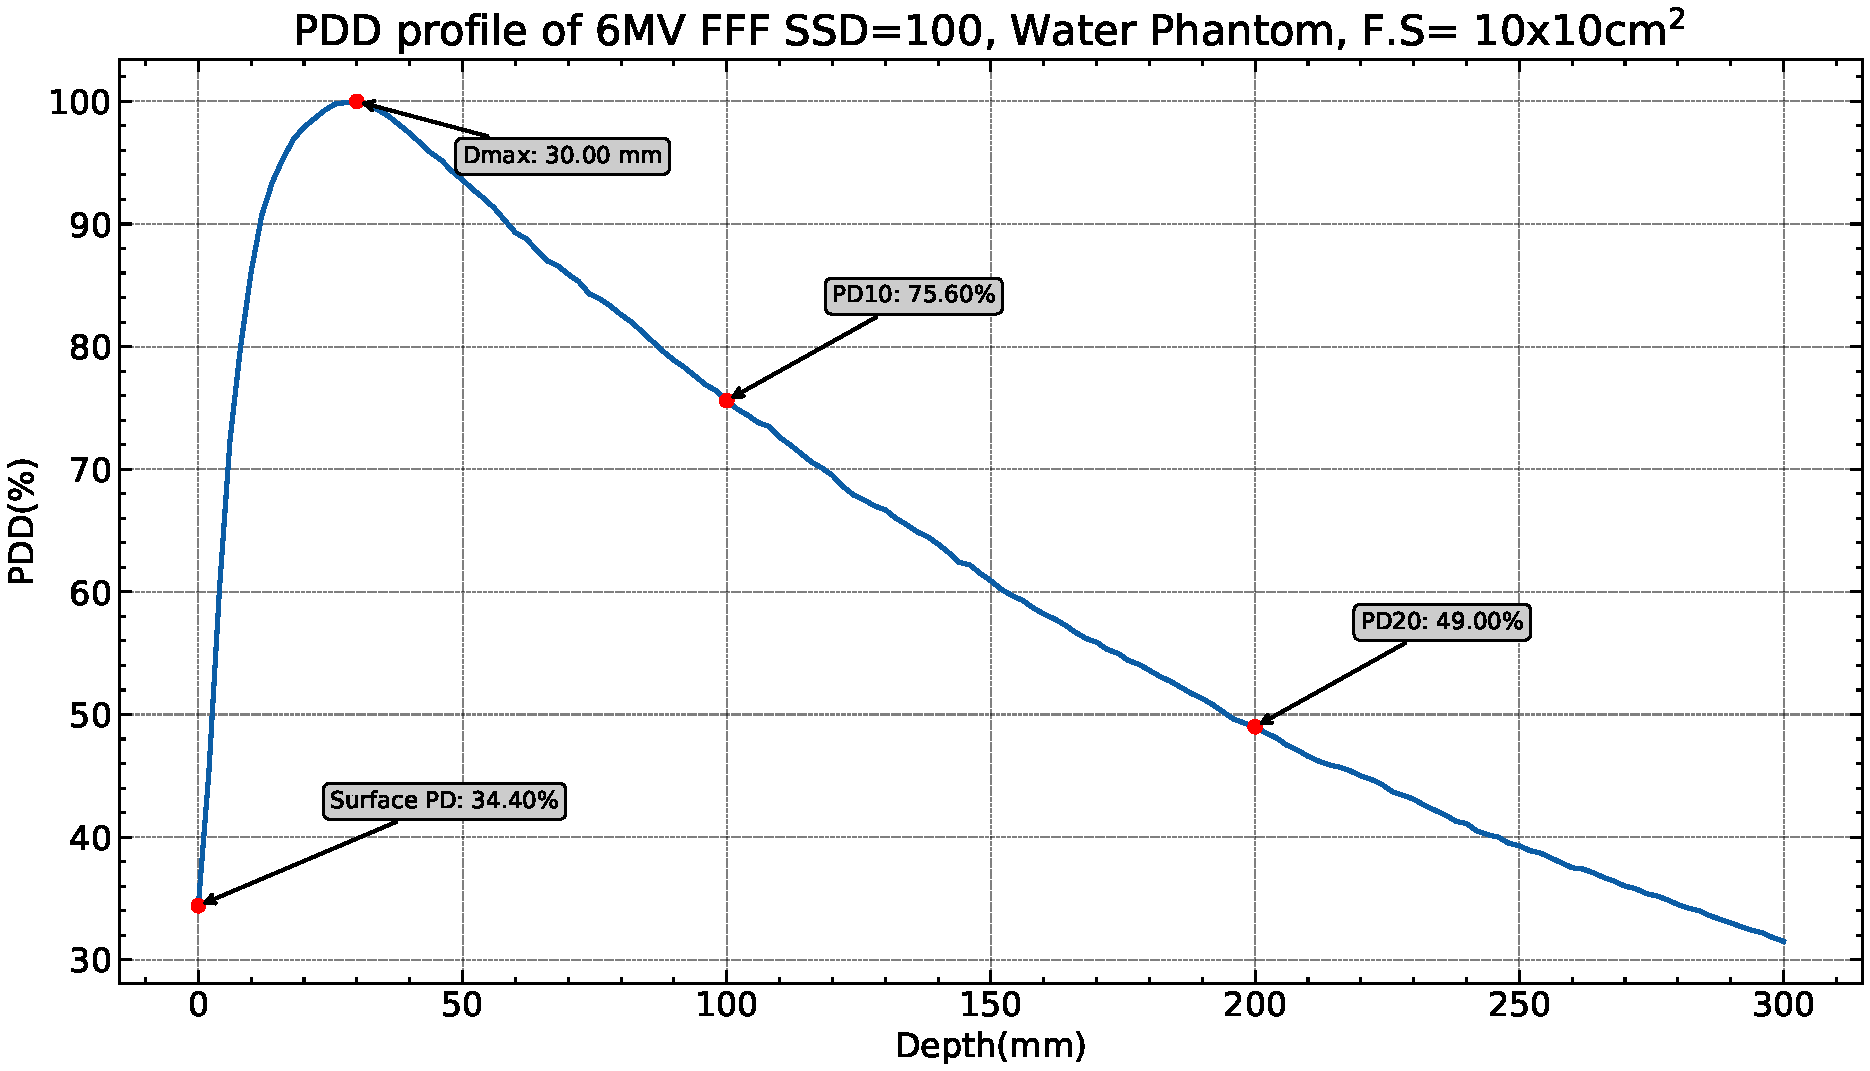
\includegraphics[width=0.8\textwidth]{Program/Figures/PDD/PDD_6MVFFFPhoton.pdf}
	\caption{Percentage depth dose for 6 MV FFF photon beam.}
\end{figure}

\begin{figure}[H]
	\centering
	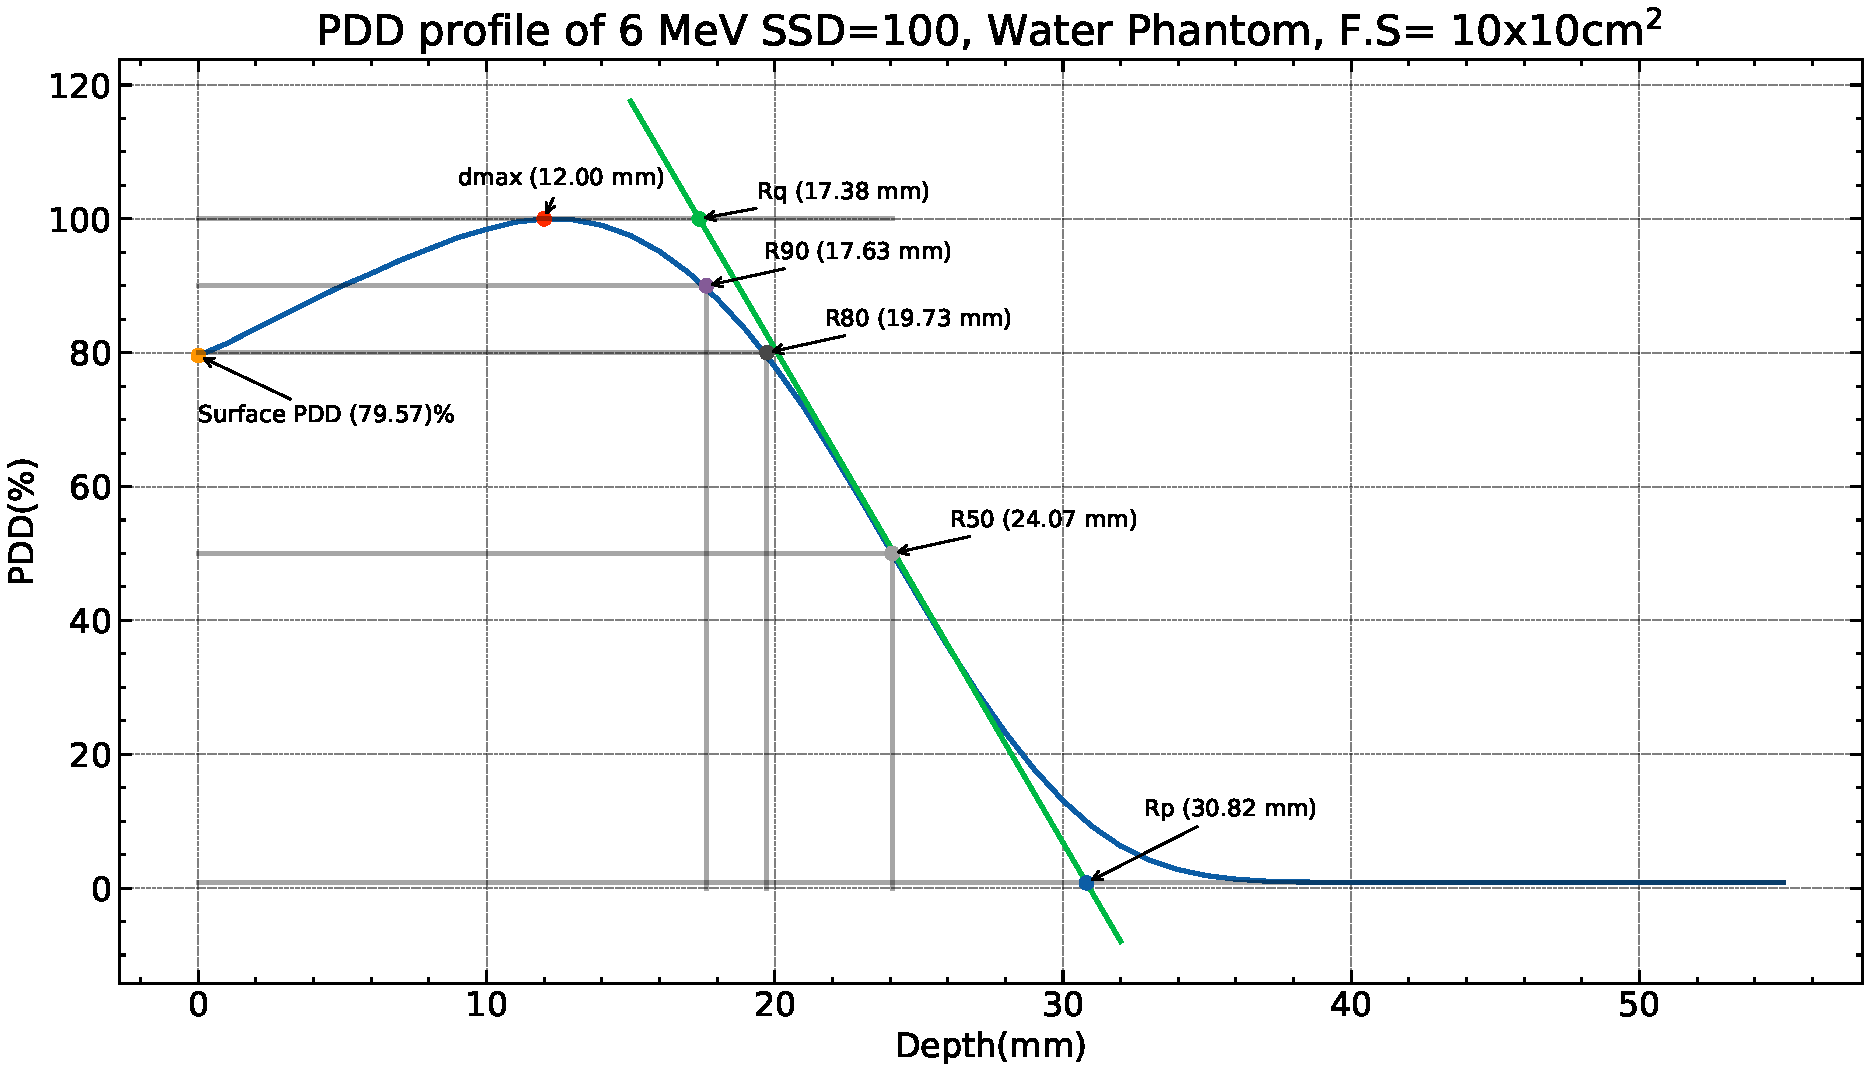
\includegraphics[width=0.8\textwidth]{Program/Figures/PDD/PDD_6MeV_Electron.pdf}
	\caption{Percentage depth dose for 6 MeV electron beam.}
\end{figure}

\clearpage
\subsection{Observed Beam Profiles}

\subsubsection{6 MV Photon (10 x 10 cm2)}

\begin{figure}[H]
	\centering
	
\includegraphics[width=0.8\textwidth]{Program/Figures/Profile/6 MV photon(10 by 10)/InlineProfile.pdf}
	\caption{Inline beam profile for 6 MV photon beam at 10 $\times$ 10 cm$^2$.}
\end{figure}

\begin{figure}[H]
	\centering
	
\includegraphics[width=0.8\textwidth]{Program/Figures/Profile/6 MV photon(10 by 10)/CrosslineProfile.pdf}
	\caption{Crossline beam profile for 6 MV photon beam at 10 $\times$ 10 cm$^2$.}
\end{figure}

\subsubsection{6 MV Photon (35 x 35 cm2)}

\begin{figure}[H]
	\centering
	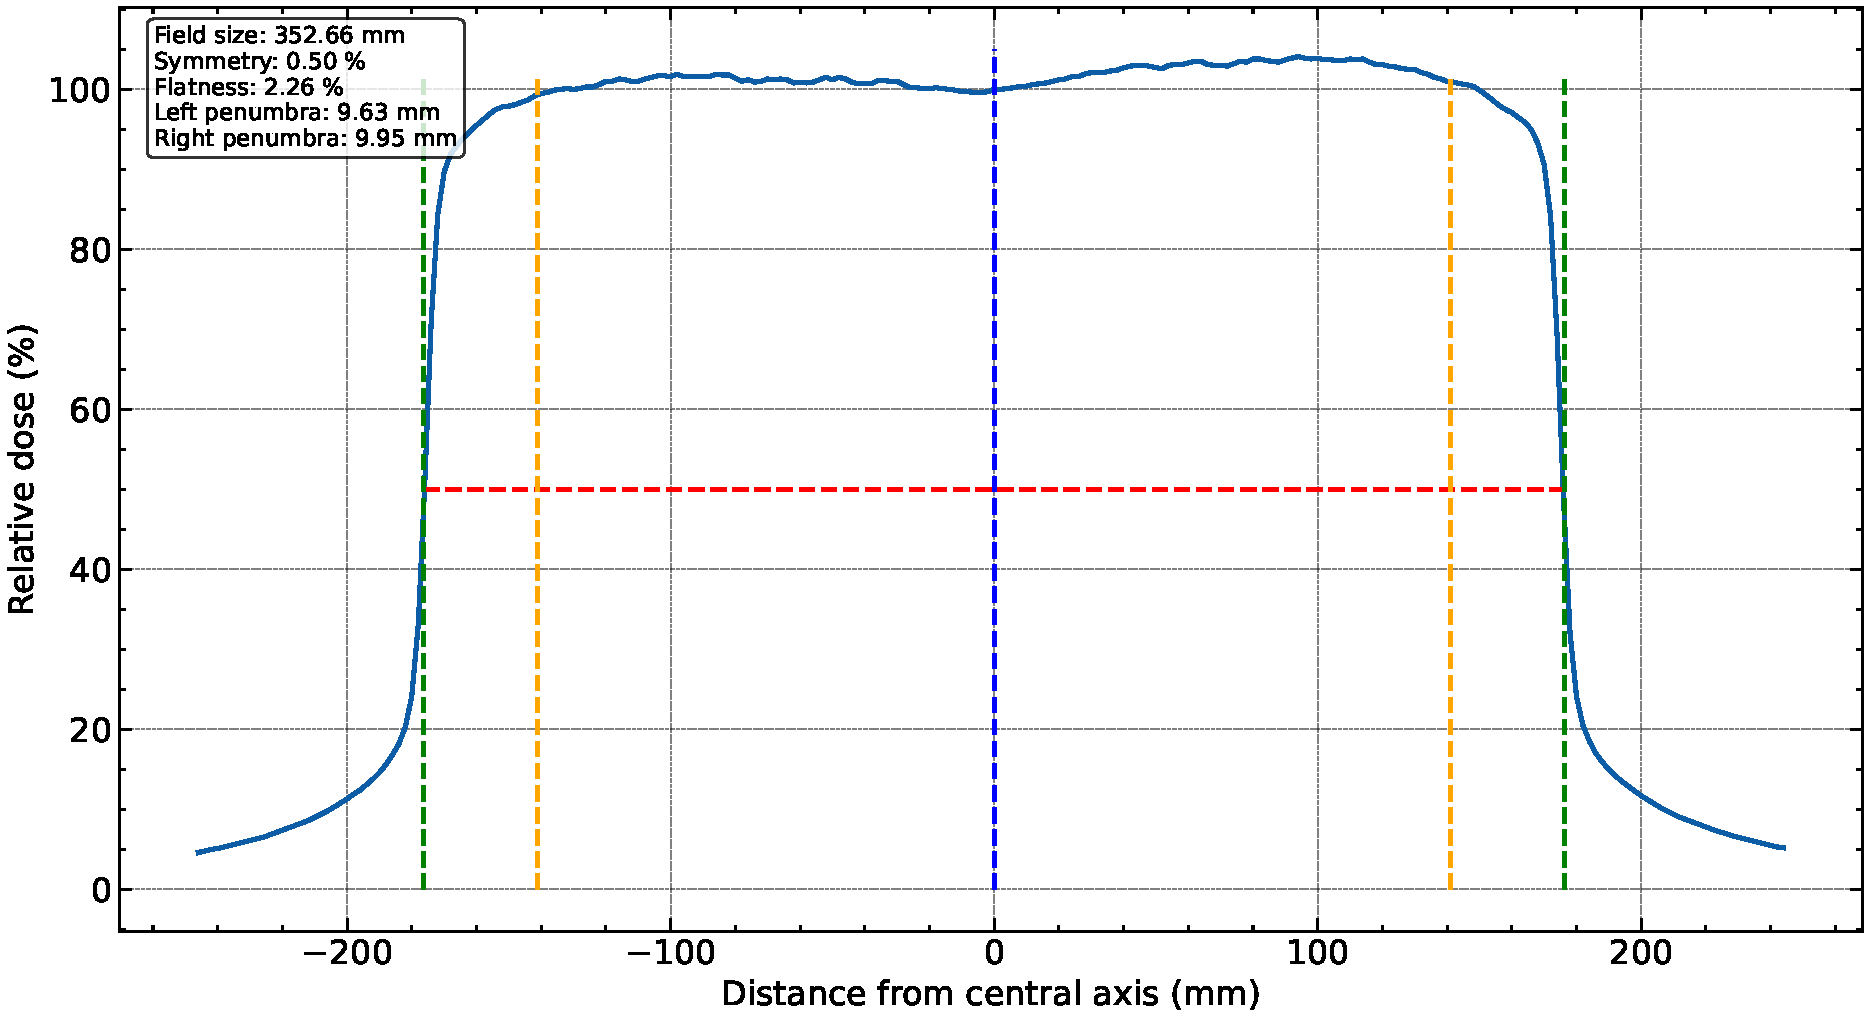
\includegraphics[width=0.8\textwidth]{Program/Figures/Profile/6 MV Photon(35 by 35)/InlineProfile.pdf}
	\caption{Inline beam profile for 6 MV photon beam at 35 $\times$ 35 cm$^2$.}
\end{figure}

\begin{figure}[H]
	\centering
	
\includegraphics[width=0.8\textwidth]{Program/Figures/Profile/6 MV Photon(35 by 35)/CrosslineProfile.pdf}
	\caption{Crossline beam profile for 6 MV photon beam at 35 $\times$ 35 cm$^2$.}
\end{figure}

\subsubsection{6 MV FFF Photon (20 x 20 cm2)}

\begin{figure}[H]
	\centering
	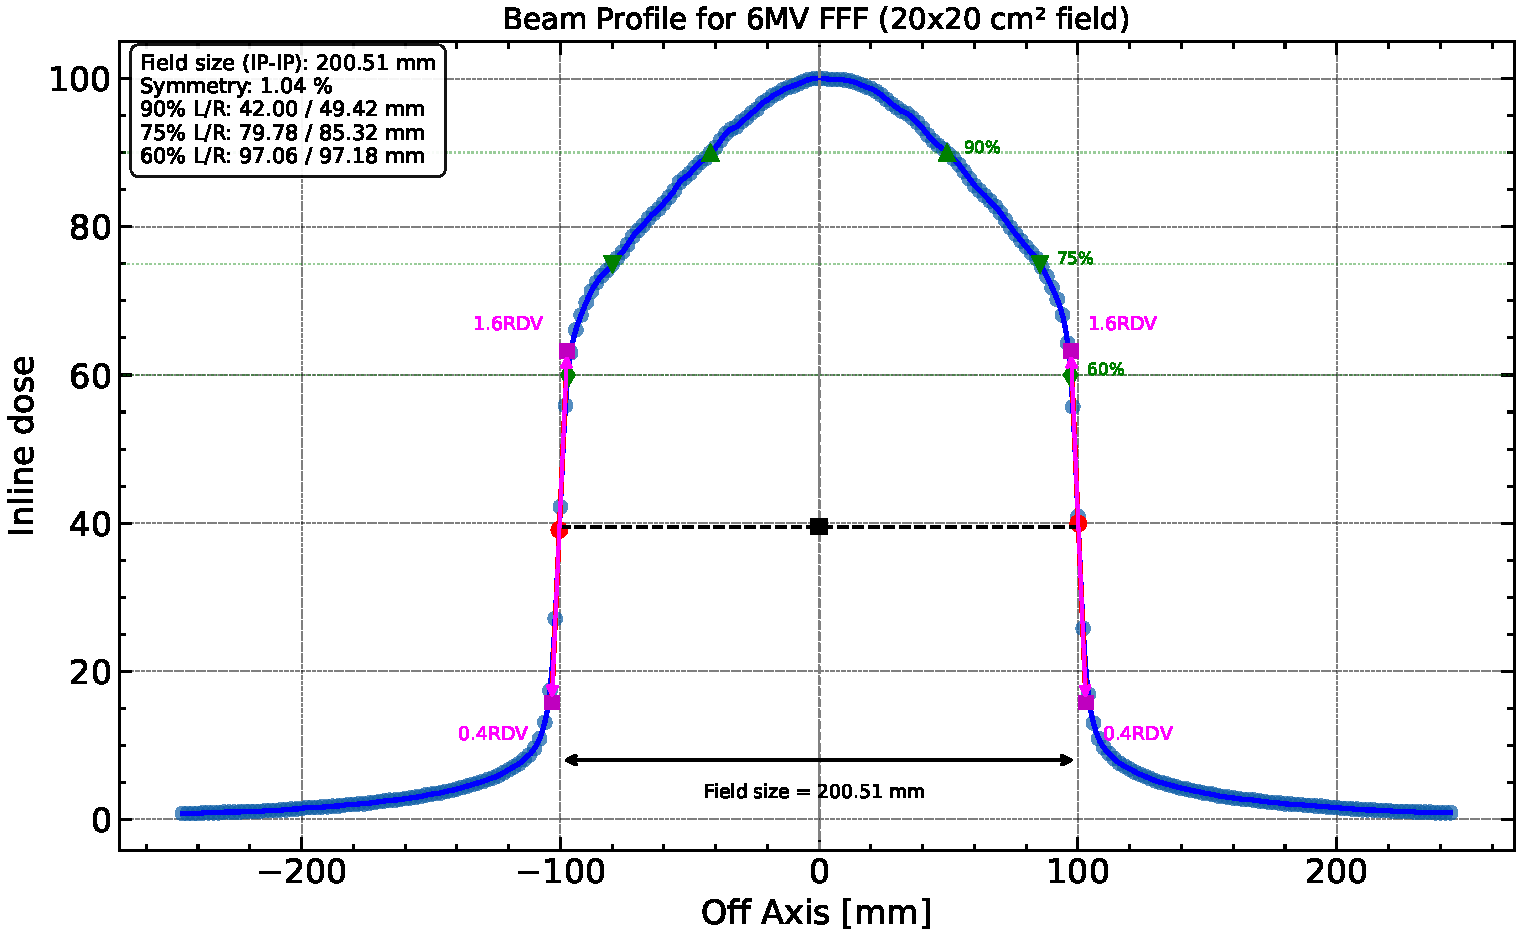
\includegraphics[width=0.8\textwidth]{Program/Figures/Profile/6MV FFF(20 by 20)/Beam_Profile_FFF.pdf}
	\caption{Inline beam profile for 6 MV FFF photon beam at 20 $\times$ 20 cm$^2$.}
\end{figure}

\begin{figure}[H]
	\centering
	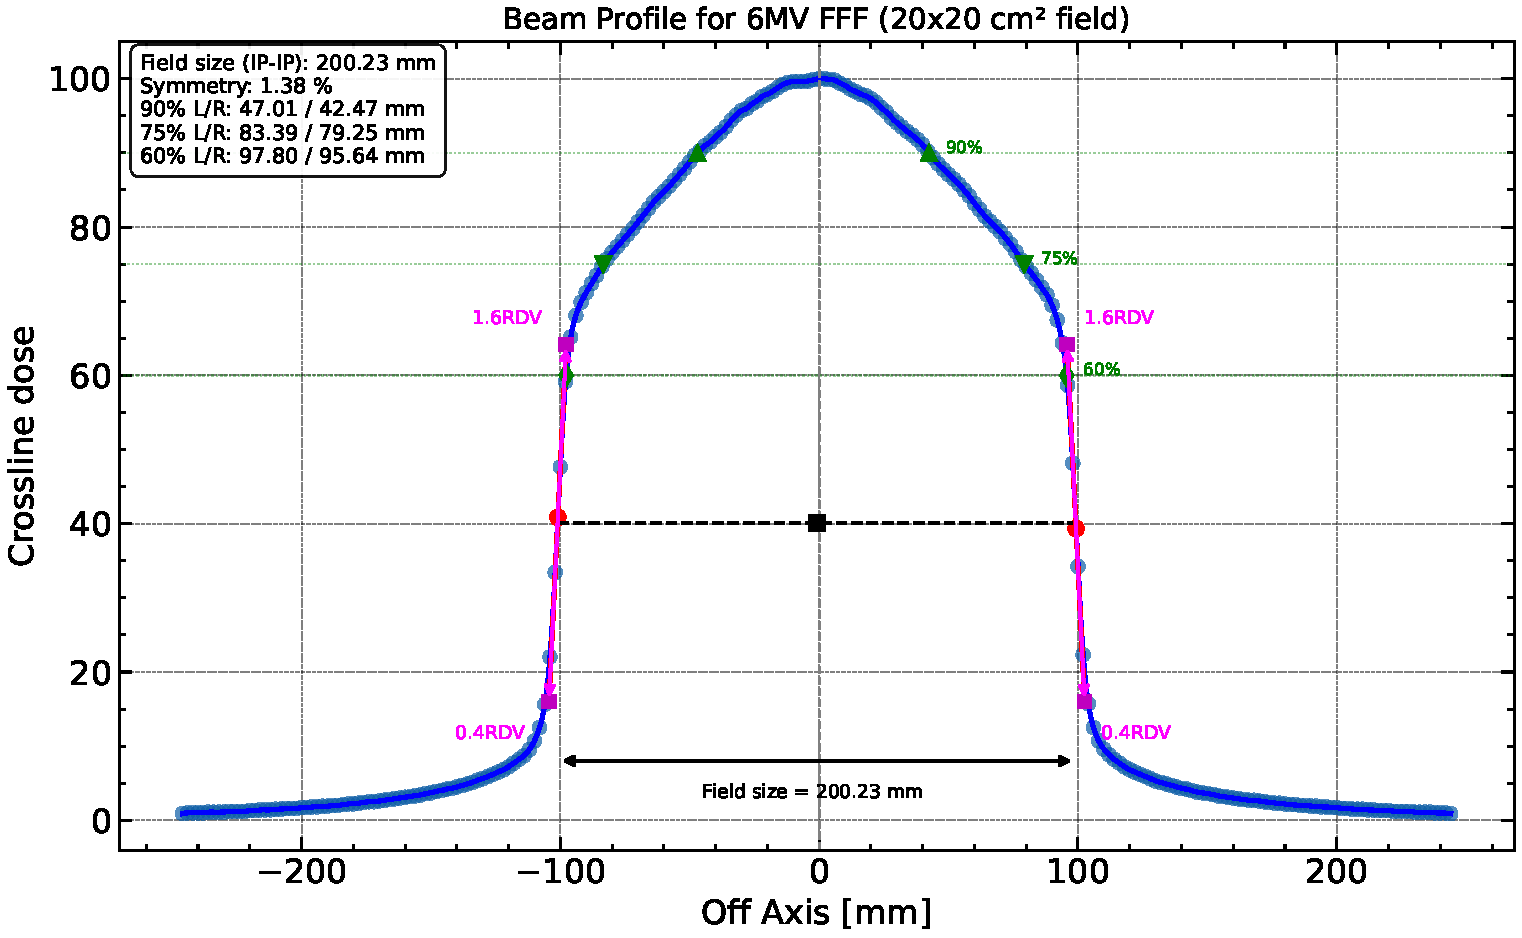
\includegraphics[width=0.8\textwidth]{Program/Figures/Profile/6MV FFF(20 by 20)/Beam_Profile_FFF_Crossline.pdf}
	\caption{Crossline beam profile for 6 MV FFF photon beam at 20 $\times$ 20 cm$^2$.}
\end{figure}

\subsubsection{6 MeV Electron (10 x 10 cm2)}

\begin{figure}[H]
	\centering
	
\includegraphics[width=0.8\textwidth]{Program/Figures/Profile/6MeV(10 by 10)/InlineProfile.pdf}
	\caption{Inline beam profile for 6 MeV electron beam at 10 $\times$ 10 cm$^2$.}
\end{figure}

\begin{figure}[H]
	\centering
	
\includegraphics[width=0.8\textwidth]{Program/Figures/Profile/6MeV(10 by 10)/CrosslineProfile.pdf}
	\caption{Crossline beam profile for 6 MeV electron beam at 10 $\times$ 10 cm$^2$.}
\end{figure}

\clearpage
\subsection{Python Programs Used for Analysis}

\lstinputlisting[style=mypython, caption={Python program for photon PDD analysis.}]{Program/PDD_Photon.py}

\lstinputlisting[style=mypython, caption={Python program for electron PDD analysis.}]{Program/PDD_Electron.py}


\lstinputlisting[style=mypython, caption={Python program for photon flattened-beam profile analysis.}]{Program/BeamProfile_Photon_FF.py}

\lstinputlisting[style=mypython, caption={Python program for FFF beam profile analysis.}]{Program/BeamProfile_FFF.py}

\lstinputlisting[style=mypython, caption={Python program for electron beam profile analysis.}]{Program/BeamProfile_Electron_FF.py}
